\chapter{Evaluation}
\label{chap:evaluation}
In diesem Kapitel wird die Trainingsqualität der generierten Kreaturen evaluiert. 

\section{Einschränkungen der Evaluation}\label{Vorlaeufige_Ergebnisse}

\subsection{Auswahl der Kreaturen}
Die Evaluation wird aufgrund der limitierten Rechenressourcen auf jeweils eine Vierbeiner Kreatur und eine Zweibeiner Kreatur beschränkt. Abbildung \ref{fig:4B_creature_settings} zeigt die Parameter zur Generierung der Vierbeiner Kreatur und Abbildung \ref{fig:4B_joint_limit_overrides} zeigt die Einstellungen zum Überschreiben der Joint Limits der generierten Vierbeiner Kreatur. Abbildung \ref{fig:2B_creature_settings} zeigt die Parameter zur Generierung der Zweibeiner Kreatur.

\begin{figure}
    \centering
    \begin{subfigure}[b]{0.45\textwidth}
        \centering
        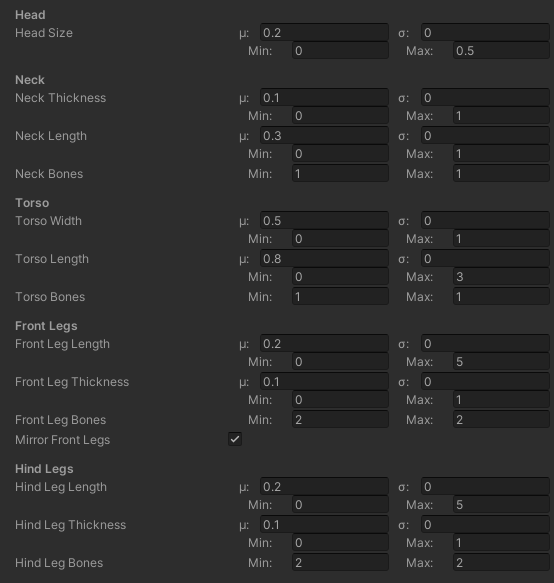
\includegraphics[width=0.95\linewidth]{resources/img/4BSettings.png}
        \caption{4B Parameter}\label{fig:4B_creature_settings}
    \end{subfigure}
    \hfill
    \begin{subfigure}[b]{0.45\textwidth}
        \centering
        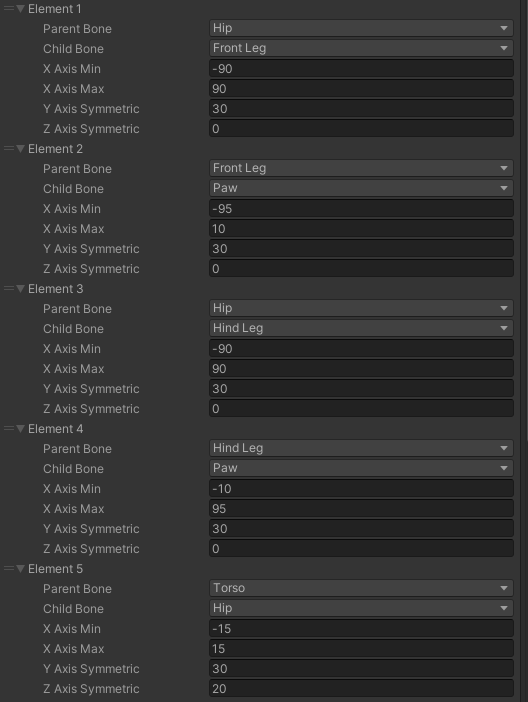
\includegraphics[width=0.95\linewidth]{resources/img/4BJointLimitOverrides.png}
        \caption{4B Joint Limit Overrides}\label{fig:4B_joint_limit_overrides}
    \end{subfigure}
\end{figure}

\paragraph{Vierbeiner-Einstellungen}
Bei der Wahl der Parameter für das Generieren des Vierbeiners war es wichtig, dass die generierte Kreatur sowohl eine gewisse Stabilität beim Laufen als auch eine ungefähre Größe von 2m hat. Um geeignete Parameter zu finden, wurden viele Vortests durchgeführt. Bei den vielen Vortest hat sich gezeigt, dass Vierbeiner, deren Beine nur aus zwei Elemente bestehen, stabiler laufen als Vierbeiner, deren Beine aus drei Elemente bestehen. Außerdem werden die standard Joint Limits des Generators für die Beine der Kreaturen überschrieben, da in den Vortests die Kreaturen mit den standard Joint Limits weder stabil laufen noch aufstehen konnten. Aus diesen Vortest ergab sich eine Basisvierbeinerkreatur, deren Beine aus zwei Elemente bestehen. In weitern Vortests wurden Variationen dieser Basisvierbeinerkreatur getestet. Bei den Variationen wurden zum Beispiel die Anzahl der Torsoknochen oder die Breite und Länge von Beinknochen verändert. Die Variationen konnten zwar alle recht stabil laufen, hatten aber Schwierigkeiten beim Aufstehen. Aufgrund der Schwierigkeiten der Variationen wurde schließlich auch die Basisvierbeinerkreatur für die finale Abgabe verwendet. 

\begin{figure}[ht]
    \centering
    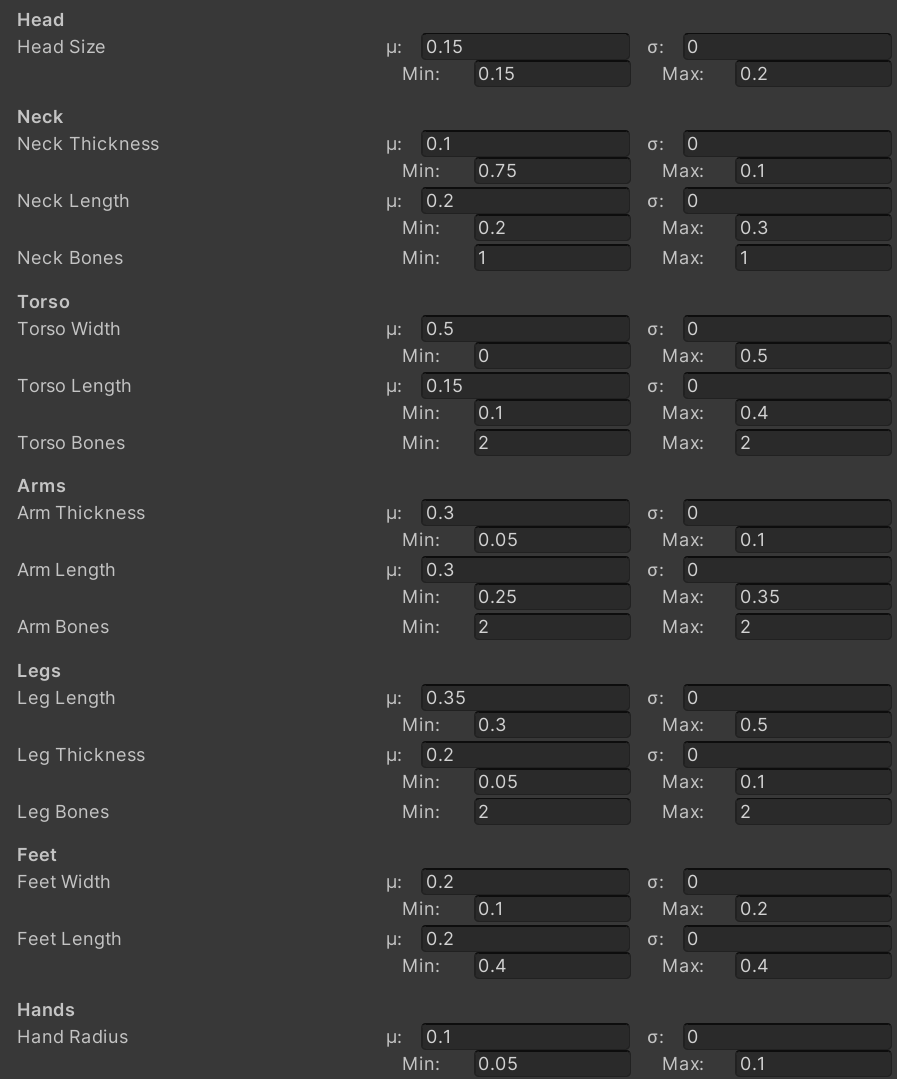
\includegraphics[width=0.5\linewidth]{resources/img/2bSettings}
    \caption{2B Parameter}
    \label{fig:2B_creature_settings}
\end{figure}

\paragraph{Zweibeiner-Einstellungen}
Da die Zweibeinerkreatuen am meisten Probleme bei der Stabilität haben, gab es keine genauen Erfahrungen zum Aufbau der Kreatur. Durch den symmetrischen Generierungsprozess und Vorüberlegungen der Kreaturen-Ersteller sollten möglichst alle generierbaren Zweibeiner im Gleichgewicht sein. Der Einstellungsprozess für die Beispielfigur reduziert sich daher auf das Reduzieren der Größe. Hierfür wurden Menschen im Raum als Vorlage genutzt, um Möglichst die Proportionen in dem Generator nachzuahmen. Die daraus resultierende Figur bestätigte sich in mehreren Vortest und wurde deshalb auch für die finale Abgabe verwendet

\subsection{Konfiguration der Trainingsdurchläufe}
Die Erfahrung während der Entwicklungsphase der Projektgruppe hat gezeigt, dass die verwendete PPO Implementierung weitestgehend robust gegenüber der verwendeten Hyperparameter ist, solange eine ausreichend große Batchgröße verwendet wird. Aufgrund der limitierten Rechenressourcen wurde deswegen auf eine Hyperparameteroptimierung verzichtet und es werden die Hyperparameter aus der Konfigurationsdatei des Walkers von ml-Agents verwendet. Abbildung \ref{fig:evaluation_config} zeigt die für die Evaluation verwendete neroRL Konfigurationsdatei. 
Für die Trainingsdurchläufe werden Unity Builds mit 16 Agenten verwendet, die auf 8 parallelen Workern ausgeführt werden. Dementsprechend werden die Daten parallel von 128 Agenten gesammelt. Jeder Agent führt bei jeder fünften Aktualisierung der Physikengine eine Aktion aus. Für das Training wird eine Batchgröße von 102400 verwendet, somit entsprechen 10 Updates etwa 1 Mio Schritten in der Umgebung.
Die in Tabelle \ref{tab:rewardfunctions} beschriebenen Reward-Funktionen für das Aufstehen und Laufen werden jeweils zwei Mal für die Vierbeinige und zwei Mal für die Zweibeinige Kreatur trainiert. Dabei werden alle 100 Updates die Policies zwischengespeichert und zum Sammeln der Evaluationsdaten verwendet. Für die Evaluation werden mit den gespeicherten Policies jeweils 128 zufällige Episoden ausgeführt und dabei Reward und Episodenlänge gesammelt.

\begin{figure}
	\centering
	\begin{subfigure}[b]{0.4\textwidth}
		\centering
		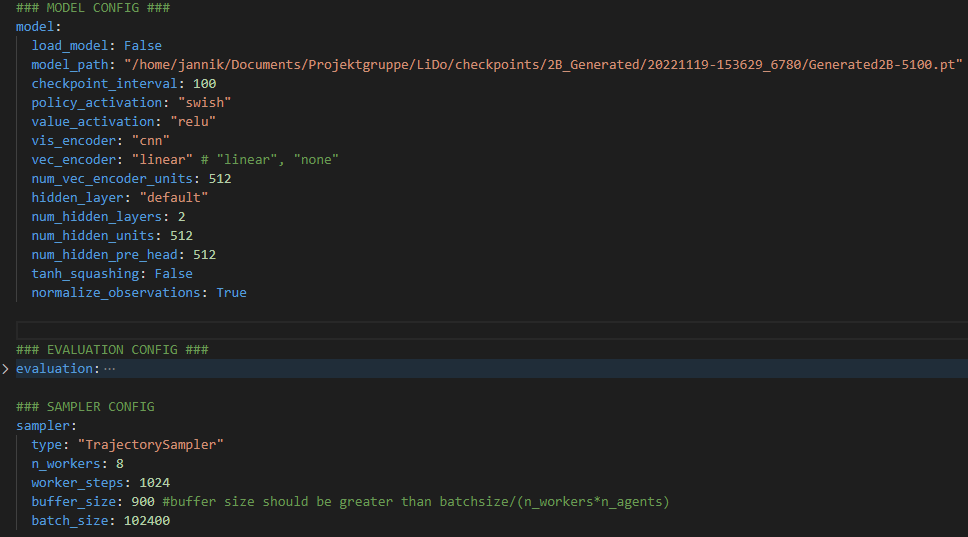
\includegraphics[width=\textwidth]{resources/img/konfig_1.png}
	\end{subfigure}
	\hfill
	\begin{subfigure}[b]{0.4\textwidth}
		\centering
		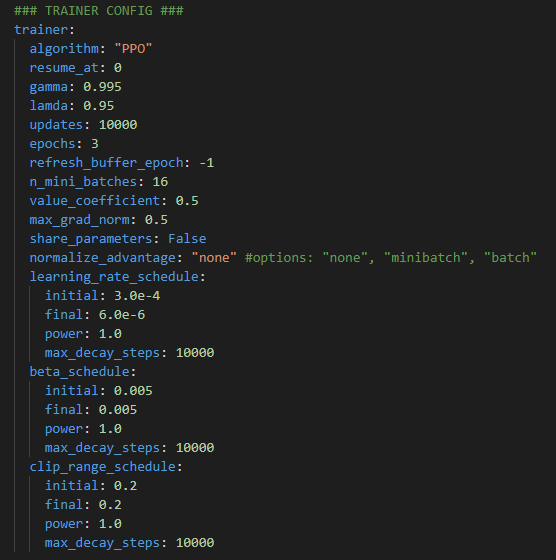
\includegraphics[width=\textwidth]{resources/img/konfig_2.png}
	\end{subfigure}
    \caption{neroRL Konfigurationsdatei für die Evaluation}\label{fig:evaluation_config}
\end{figure}

\section{Ergebnisse}
\label{ErgebnisseTraining}
In diesem Abschnitt werden die Ergebnisse der Trainingsdurchläufe für die Vierbeiner und Zweibeiner Kreaturen beschrieben. Zunächst werden Daten bezüglich des Rewards und der Länge der Trainingsepisoden analysiert. Anschließend wird die Qualität der Trainingsergebnisse bei der visuellen Evaluation in Unity beschrieben.

\subsection{Vierbeiner Kreatur}

\subsubsection{Laufen}
Die Entwicklung des Rewards beim Trainieren des Laufens der Vierbeiner Kreatur ist in Abbildung \ref{fig:Walking4B_Reward} abgebildet. Der Reward steigt in den ersten 1000 Updates deutlich an und erreicht ein Maximum von 14000. Danach fällt der Reward langsam ab auf ca. 7000-1000, ein Policy Collapse tritt nicht ein. 

\begin{figure}[ht]
    \centering
    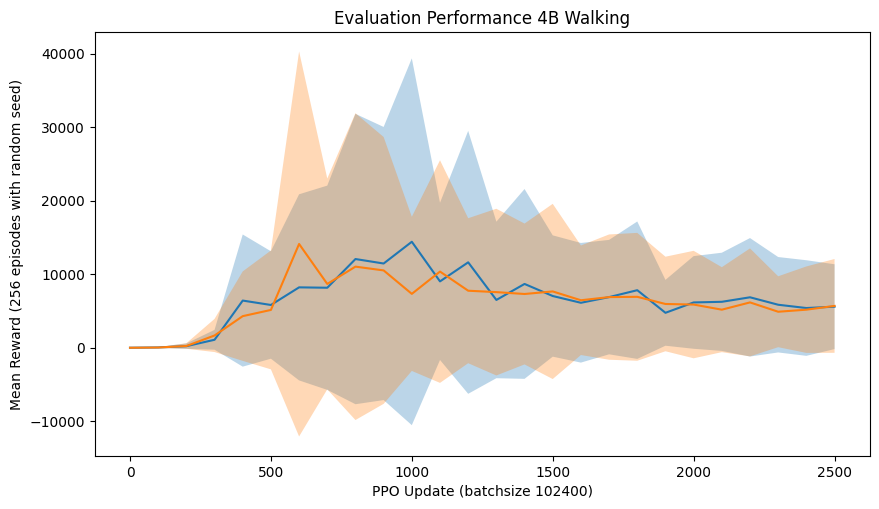
\includegraphics[width=0.5\linewidth]{resources/img/results/Walking4B_Reward.png}
    \caption{Walking 4B Reward}\label{fig:Walking4B_Reward}
\end{figure}
Die Episodenlänge der Vierbeiner beim Laufen ist unbeschränkt, eine Episode wird beendet, wenn die Kreatur mit einem Körperteil außer den Füßen den Boden berührt. Da alle 5 Physik-Aktualisierungen der Unity Umgebung eine Aktion des Agenten angefordert wird und die Unity Umgebung mit 120 Aktualisierungen pro Sekunde ausgeführt wird, entspricht eine Länge von 1000 ca. 41.5 Sekunden. Abbildung \ref{fig:Walking4B_Length} zeigt die Entwicklung der Episodenlänge während der Trainingsdurchläufe. Analog zum Reward steigt die durchschnittliche Episodenlänge in den ersten 1000 Updates deutlich an und stagniert danach bzw. fällt langsam ab. Das Maximum wird mit einer Episodenlänge von ca. 6000, umgerechnet ca. 4 Minuten und 9 Sekunden, erreicht.

\begin{figure}[ht]
    \centering
    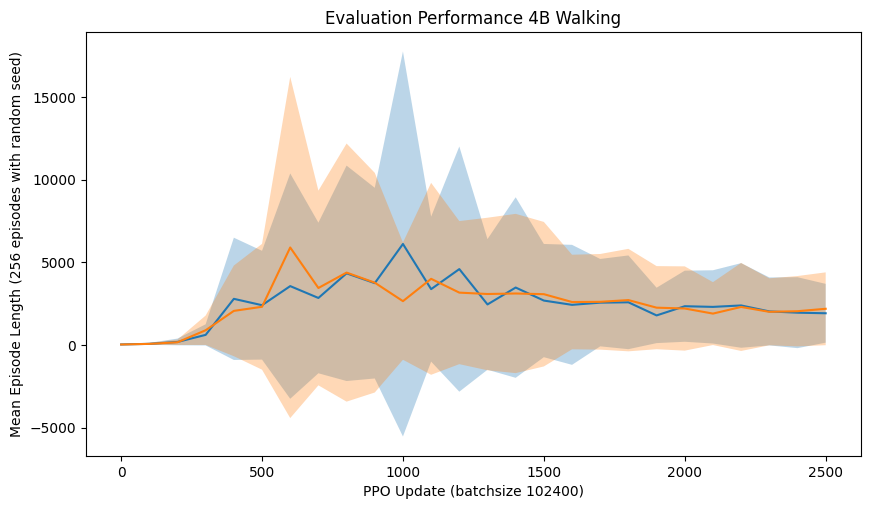
\includegraphics[width=0.5\linewidth]{resources/img/results/Walking4B_Length.png}
    \caption{Walking 4B Length}\label{fig:Walking4B_Length}
\end{figure}

Die Visuelle Evaluation in Unity zeigt, dass die Vierbeiner Kreatur mit beliebigen Policies ab ca. 500 Updates weitestgehend stabil läuft. Instabilität tritt insbesondere dann auf, wenn die Kreatur mit hoher Geschwindigkeit einen Wegpunkt erreicht und eine große Drehung in Richtung des nächsten Wegpunkts durchführen muss.\newline
In Abbildung \ref{fig:4BLaufen} werden die 3 Schritte des Laufzyklus eines Vierbeiners dargestellt. Am Anfang des Zyklus springt der Vierbeiner ab (siehe \ref{fig:4B_Absprung}) und streckt während des Sprungs seine Vorderbeine nach vorne und breitet seine Hinterbeine aus (siehe \ref{fig:4B_Schritt}). Abschließend landet der Vierbeiner wieder auf seinen Beinen (siehe \ref{fig:4B_Landen}) und bereitet sich auf den nächsten Absprung vor. Das Springen des Vierbeiners beim Laufen trägt zu der oben genannten Instabilität bei.

\begin{figure}
	\centering
	\begin{subfigure}[b]{0.3\textwidth}
		\centering
		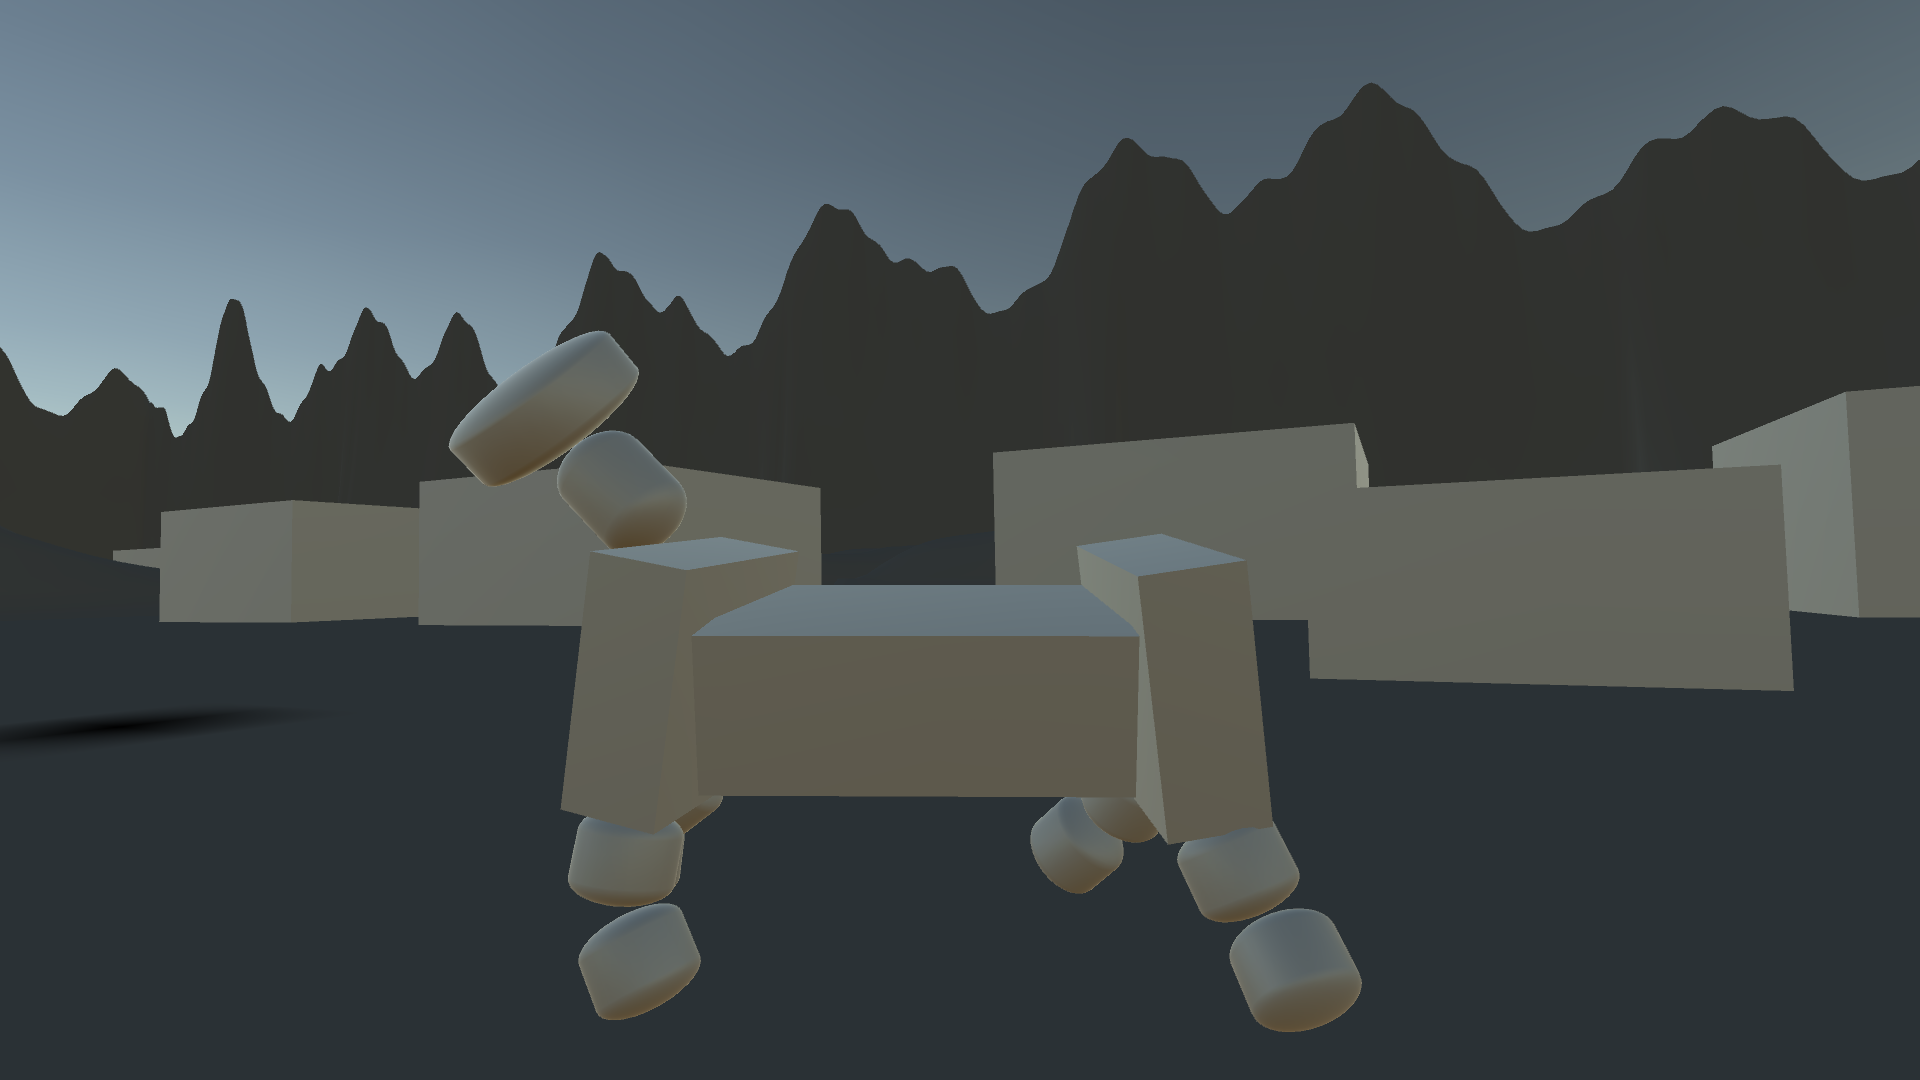
\includegraphics[width=\textwidth]{resources/img/4B_Absprung.png}
		\caption{Absprung}
		\label{fig:4B_Absprung}
	\end{subfigure}
	\hfill
	\begin{subfigure}[b]{0.3\textwidth}
		\centering
		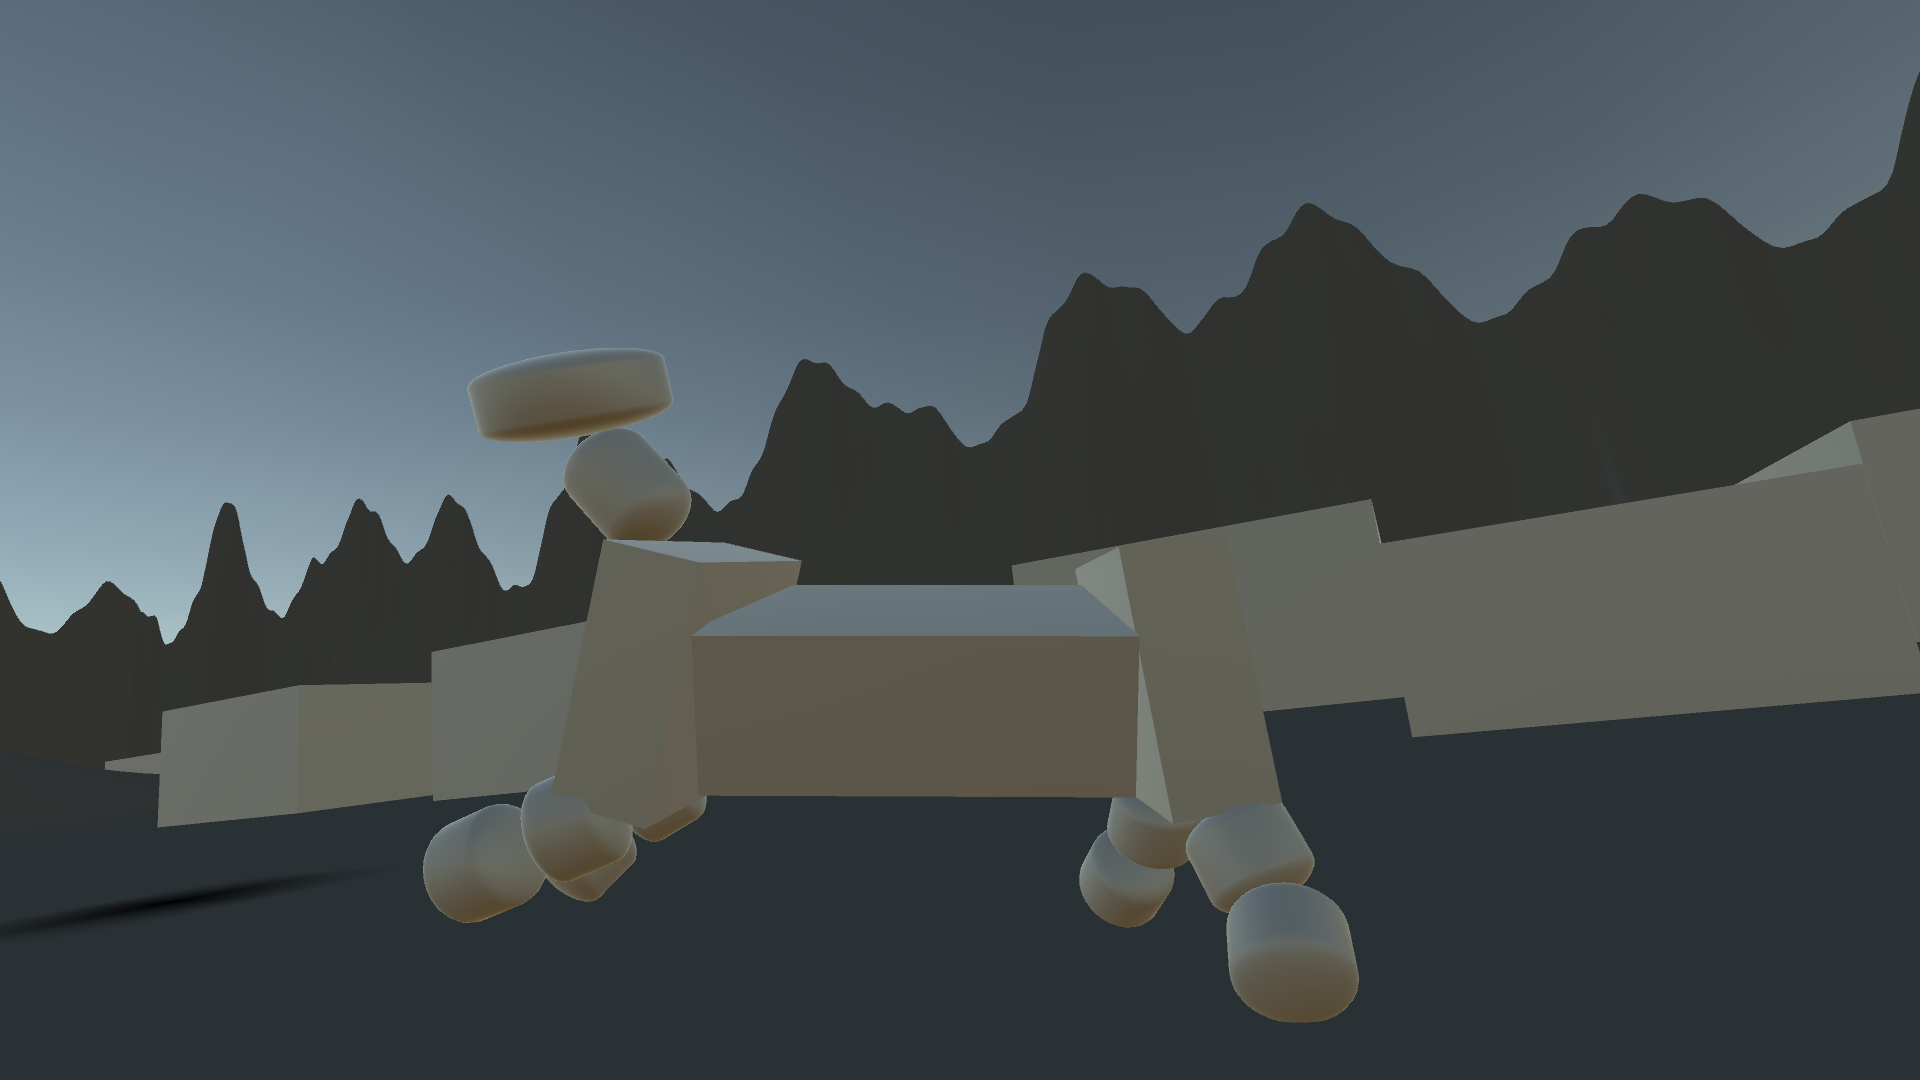
\includegraphics[width=\textwidth]{resources/img/4B_Schritt.png}
		\caption{Schritt}
		\label{fig:4B_Schritt}
	\end{subfigure}
	\hfill
	\begin{subfigure}[b]{0.3\textwidth}
		\centering
		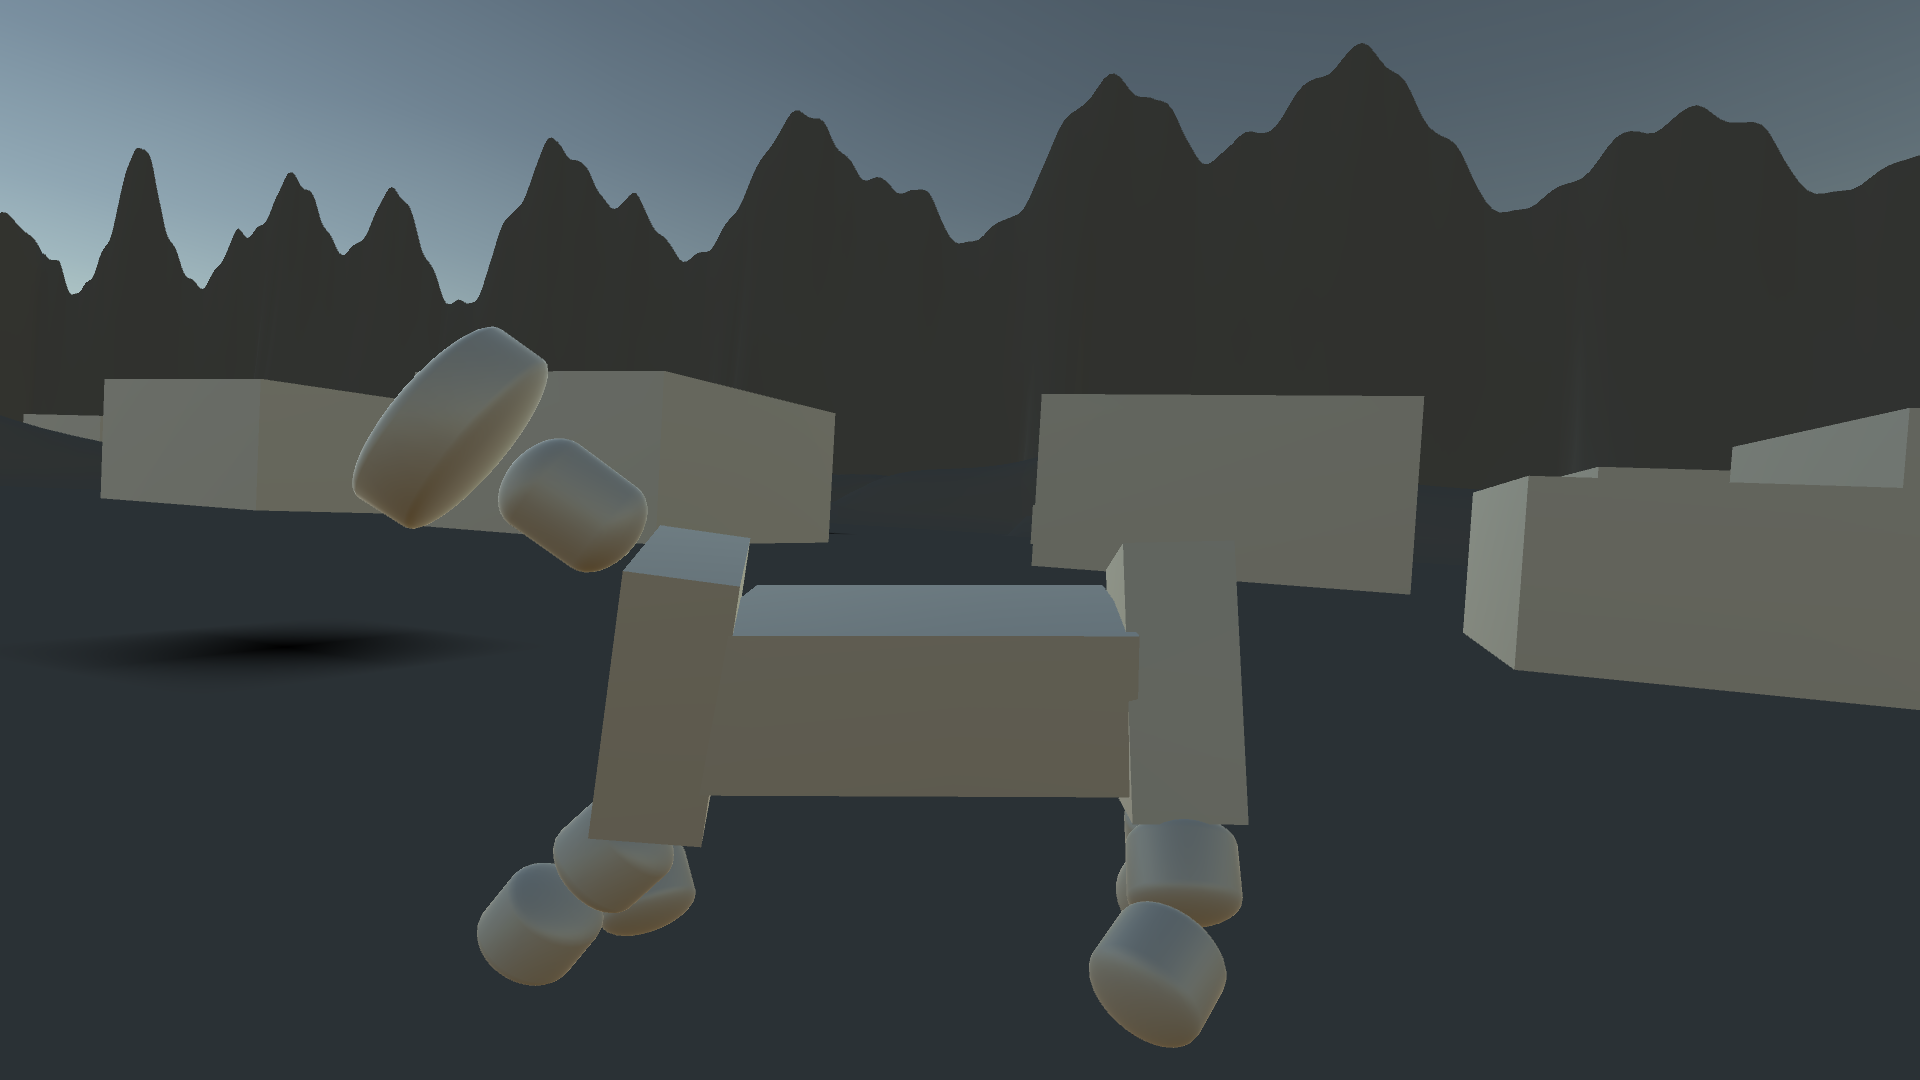
\includegraphics[width=\textwidth]{resources/img/4B_Landen.png}
		\caption{Landen}
		\label{fig:4B_Landen}
	\end{subfigure}
	\caption{3 Schritte im Laufzyklus eines Vierbeiners.}
	\label{fig:4BLaufen}
\end{figure}

\subsubsection{Aufstehen}
Abbildung \ref{fig:Standup4B_Reward} zeigt die Entwicklung des Rewards während der Updates des Trainingsdurchlaufs. Der Reward steigt in den ersten 250 Updates deutlich von 0 auf ca. 1700. Das Training stagniert für mehrere hundert Updates bei ca. 1700, bevor ein Performance Collapse eintritt, von dem sich die Policy nicht erneut erholt.

\begin{figure}[ht]
    \centering
    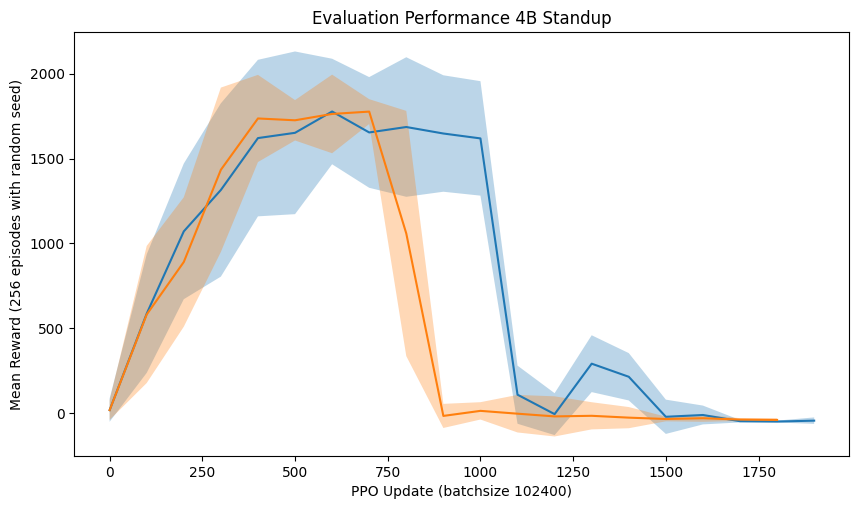
\includegraphics[width=0.5\linewidth]{resources/img/results/Standup4B_Reward.png}
    \caption{Standup 4B Reward}\label{fig:Standup4B_Reward}
\end{figure}

Die Episodenlänge für das Aufstehen der Vierbeiner ist auf 1000 Schritte beschränkt und es gibt keine Bedingung, die den Start einer neuen Episode vor Ablauf der Schritte bedingt. Da alle 5 Schritte eine Aktion des Agenten angefordert wird, liegen die in Abbildung \ref{fig:Standup4B_Length} dargestellten Episodenlängen konstant bei 201 Schritten.

\begin{figure}[ht]
    \centering
    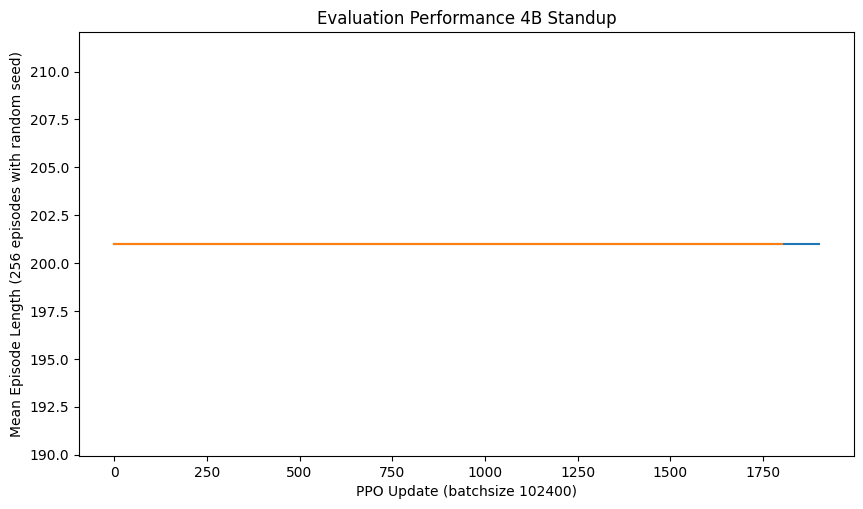
\includegraphics[width=0.5\linewidth]{resources/img/results/Standup4B_Length.png}
    \caption{Standup 4B Length}\label{fig:Standup4B_Length}
\end{figure}

Die Visuelle Evaluation in Unity zeigt, dass beliebige Policies aus den Update-Bereichen, in denen der Reward bei ca. 1700 stagniert, in der Lage sind den Vierbeiner erfolgreich aus einer liegenden Startposition aufstehen zu lassen. Die Policies nach dem Performance Collapse führen nur minimal wahrnehmbare Aktionen aus und die Kreatur bleibt unbewegt liegen.\newline
Die Abbildung \ref{fig:4BAufstehen} zeigt drei Schritte des Aufstehzyklus eines Vierbeiners. In der Abbildung \ref{fig:4B_Liegend} befindet sich die Vierbeinerkreatur in der liegenden Startposition auf dem Boden. Die Kreatur richtet sich über die Seite auf (siehe \ref{fig:4B_im_aufstehen}) und bleibt abschließend relativ stabil auf den Beinen stehen (siehe \ref{fig:4B_Stehend}).

\begin{figure}
	\centering
	\begin{subfigure}[b]{0.3\textwidth}
		\centering
		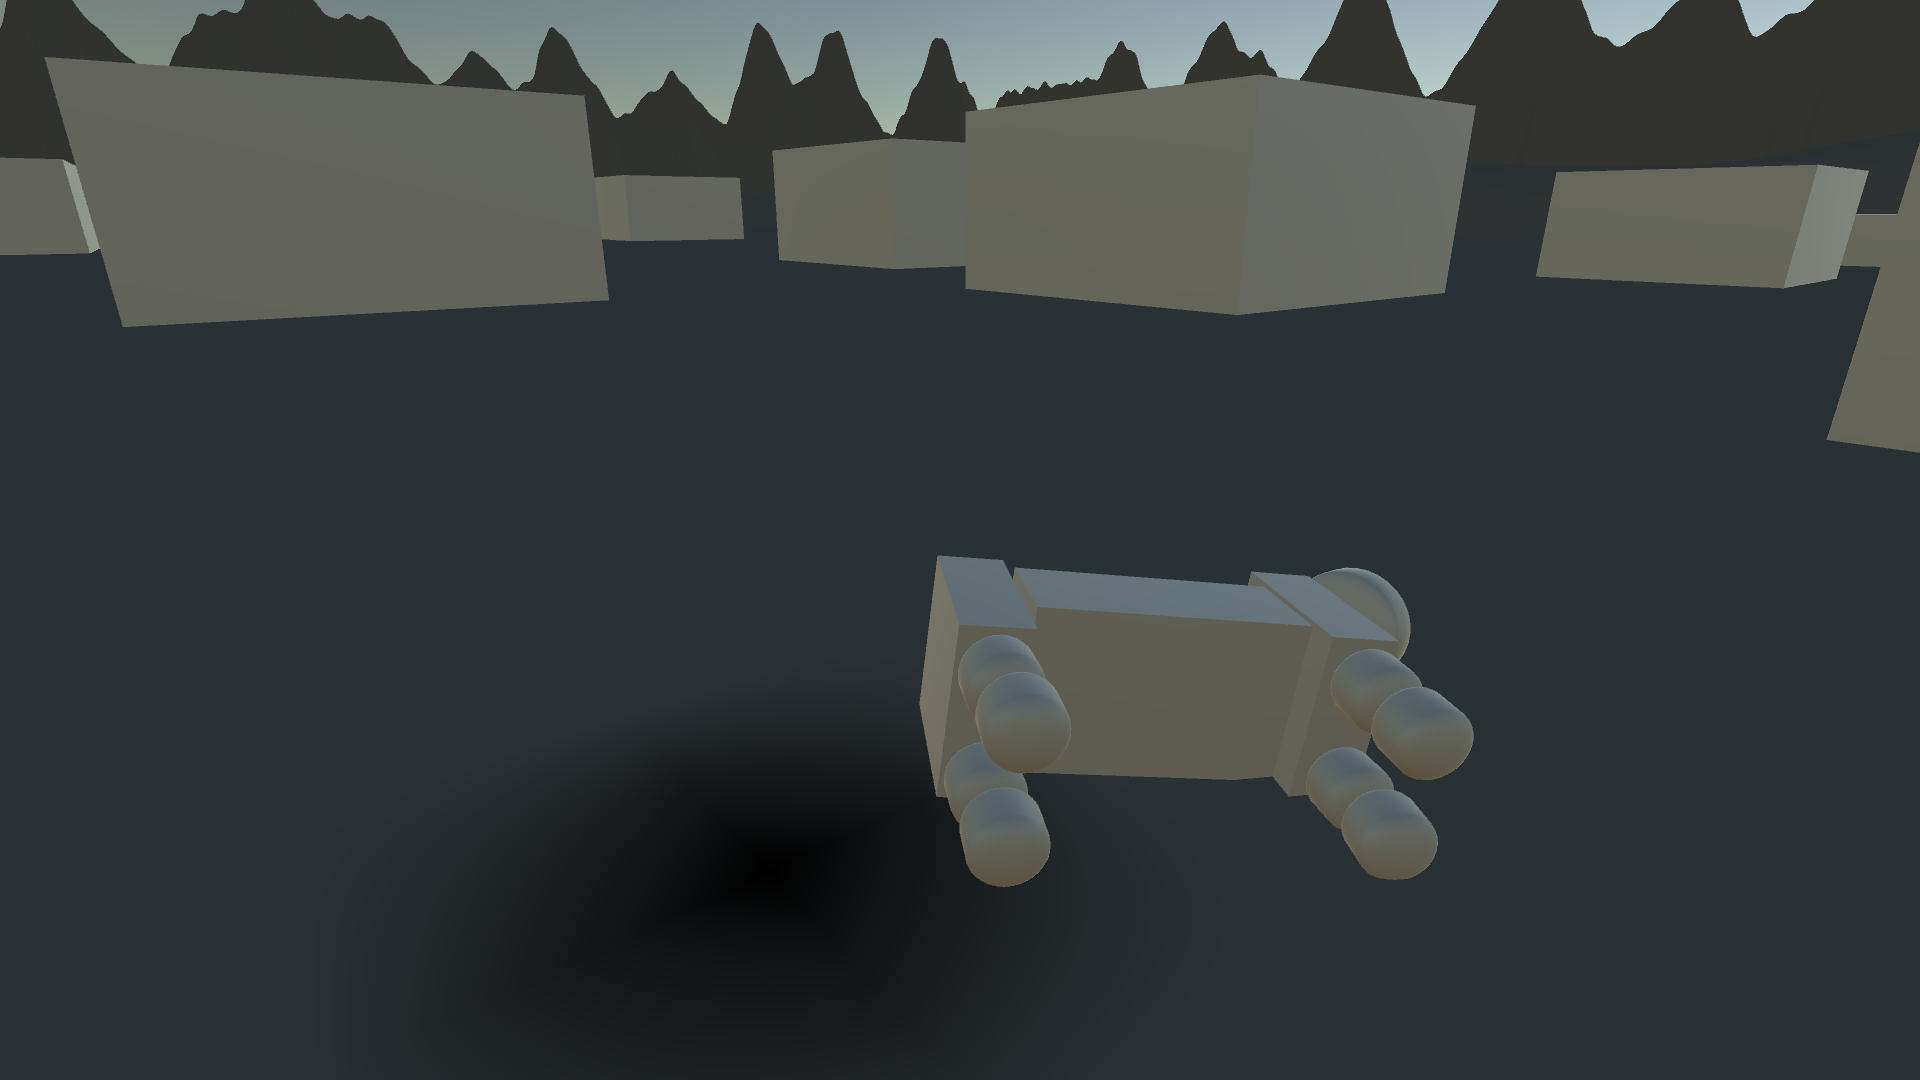
\includegraphics[width=\textwidth]{resources/img/4B_Liegend.png}
		\caption{Liegend}
		\label{fig:4B_Liegend}
	\end{subfigure}
	\hfill
	\begin{subfigure}[b]{0.3\textwidth}
		\centering
		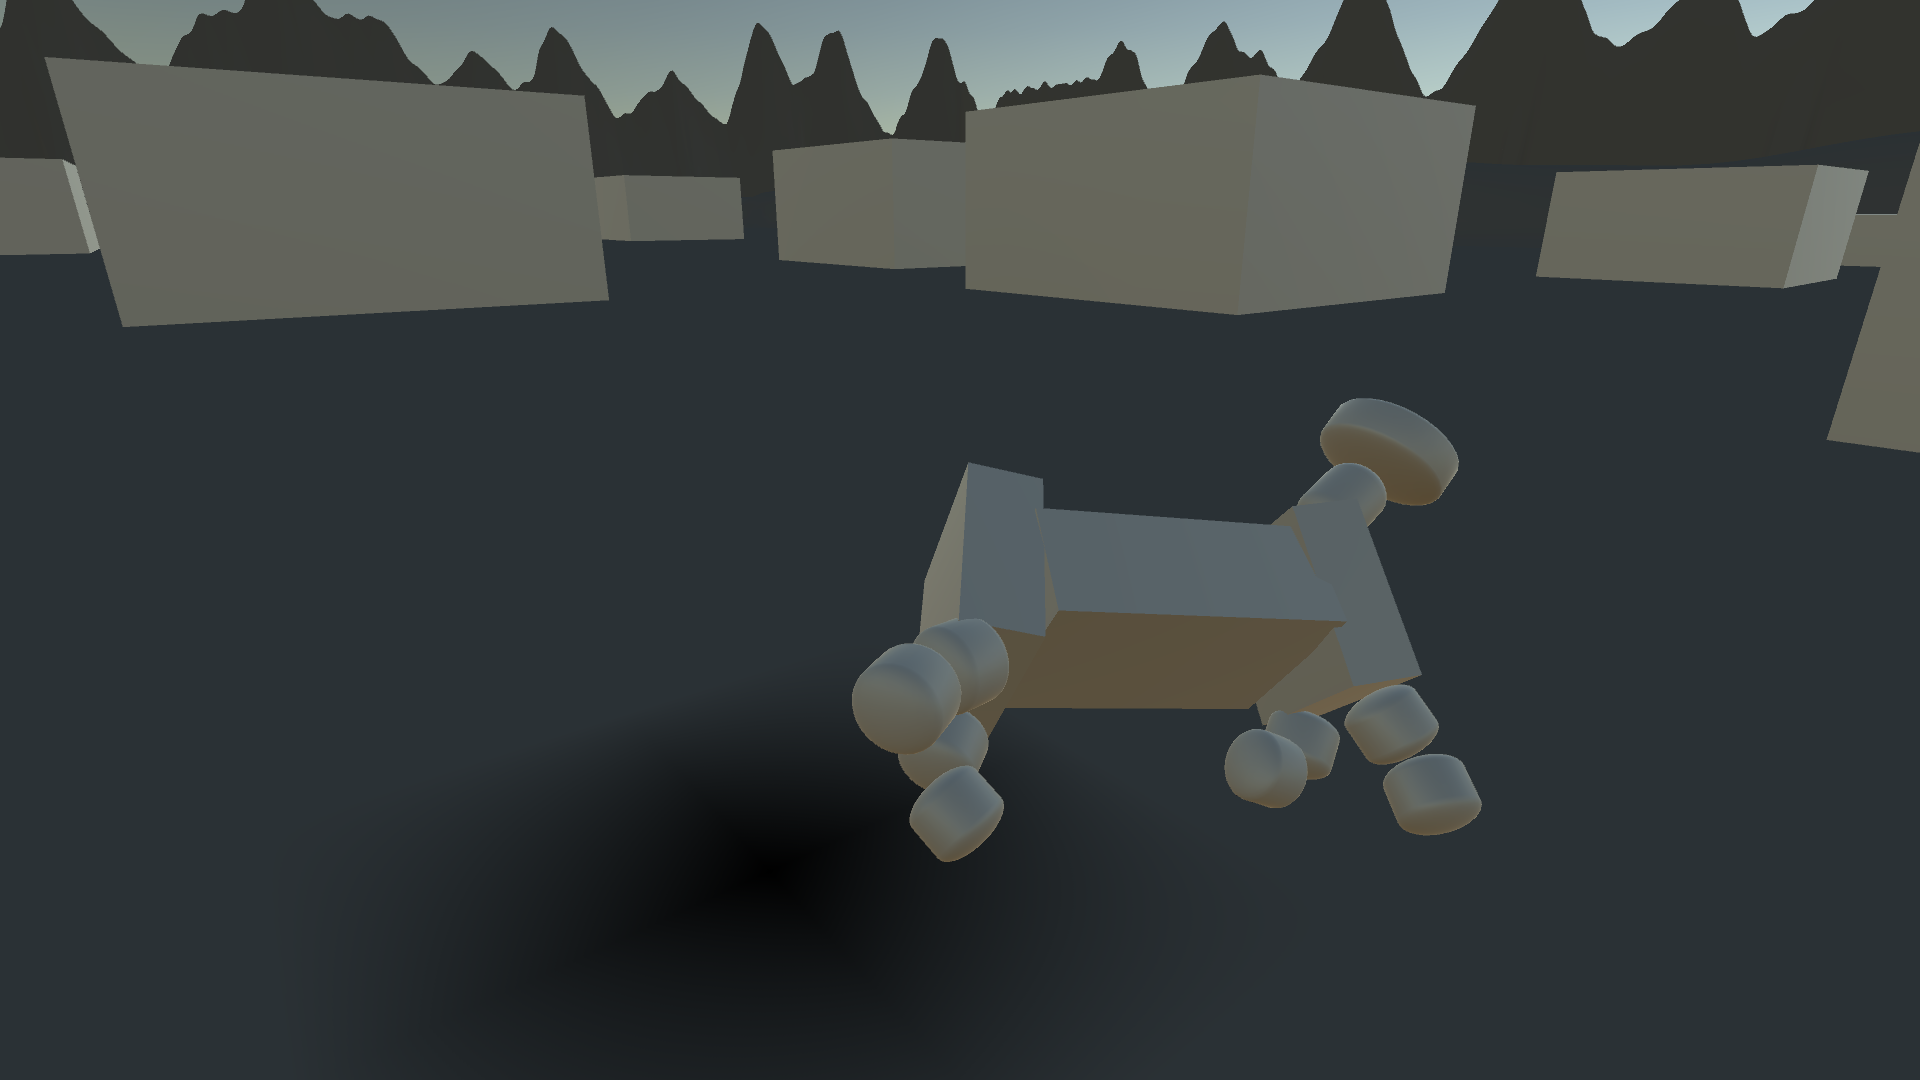
\includegraphics[width=\textwidth]{resources/img/4B_Im_Aufstehen.png}
		\caption{während des Aufstehens}
		\label{fig:4B_im_aufstehen}
	\end{subfigure}
	\hfill
	\begin{subfigure}[b]{0.3\textwidth}
		\centering
		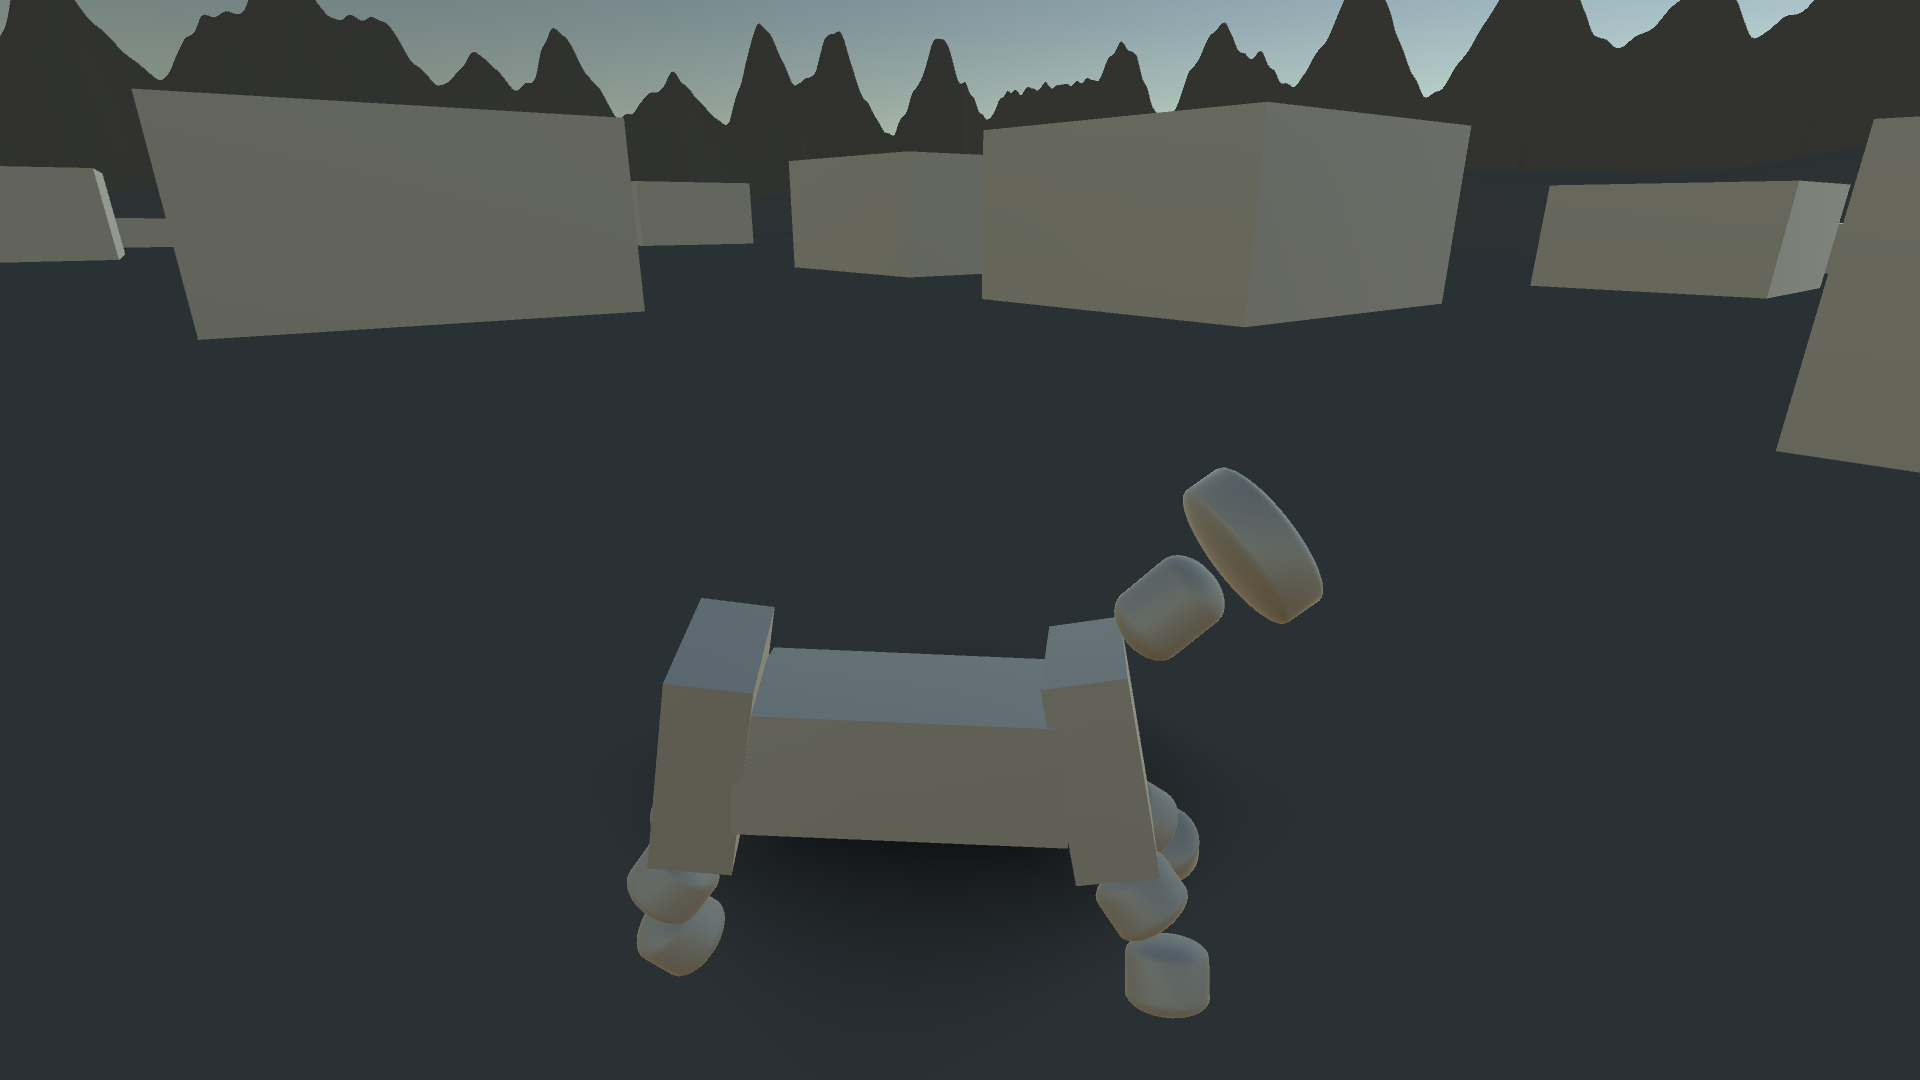
\includegraphics[width=\textwidth]{resources/img/4B_Stehend.png}
		\caption{Stehend}
		\label{fig:4B_Stehend}
	\end{subfigure}
	\caption{3 Schritte im Aufstehzyklus eines Vierbeiners.}
	\label{fig:4BAufstehen}
\end{figure}

\subsection{Zweibeiner Kreatur}

\subsubsection{Laufen}
Abbildung \ref{fig:Walking2B_Reward} zeigt die Entwicklung des Rewards beim Trainieren des Laufens der Zweibeiner Kreatur. Der Reward steigt über die ersten ca. 1500 Updates von 0 auf ca. 3000-4000 deutlich an. Danach ist steigt der Reward langsam weiter und schwankt dabei stark. In den Trainingsdurchläufen der Evaluation wurde ein maximaler Reward von ca. 5300 erreicht.

\begin{figure}[ht]
    \centering
    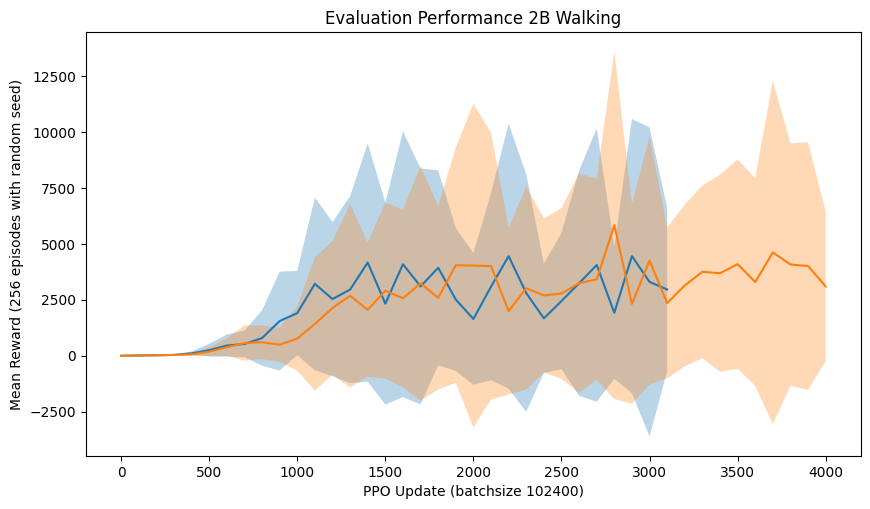
\includegraphics[width=0.5\linewidth]{resources/img/results/Walking2B_Reward.png}
    \caption{Walking 2B Reward}\label{fig:Walking2B_Reward}
\end{figure}

Die Episodenlänge der Zweibeiner beim Laufen ist nicht beschränkt. Eine Episode wird beendet, wenn die Kreatur mit einem Körperteil außer den Füßen den Boden berührt. Die in Abbildung \ref{fig:Walking2B_Length} dargestellte Episodenlänge steigt parallel zum Reward in den ersten 1500 Updates deutlich von 0 auf ca. 1000 und stagniert danach mit Schwankung. Da alle 5 Schritte eine Aktion des Agenten angefordert wird, bedeutet dies ca. 5000 Schritte. Die maximale durchschnittliche Episodenlänge beträgt ca. 2000.

% TODO Ab hier hat Nils dran rumgepfuscht 
\begin{figure}[ht]
    \centering
    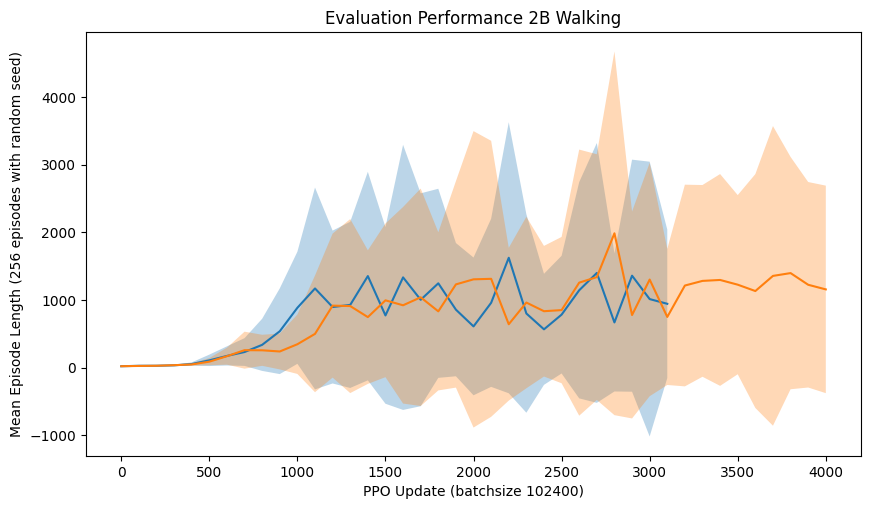
\includegraphics[width=0.5\linewidth]{resources/img/results/Walking2B_Length.png}
    \caption{Walking 2B Length}\label{fig:Walking2B_Length}
\end{figure}

Die Visuelle Evaluation in Unity zeigt, dass die Policies mit höchstem Reward den Zweibeiner laufen lassen. In Abbildung \ref{fig:2BLaufen} wird ein Laufschritt auf gerade ebene mit einer Geschwindigkeit von $5$ dargestellt.
\begin{figure}
	\centering
	\begin{subfigure}[b]{0.3\textwidth}
		\centering
		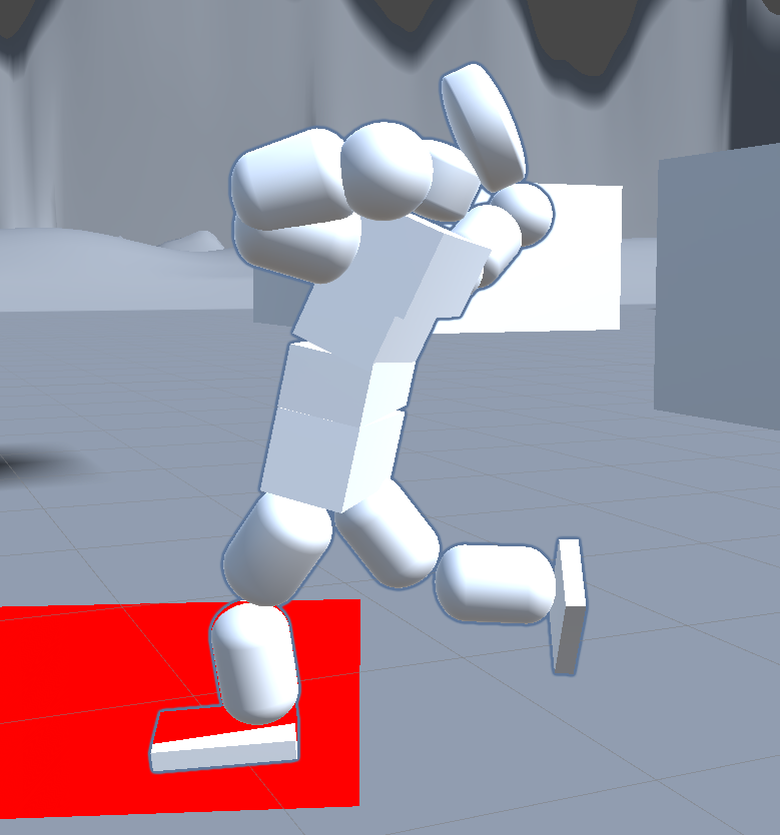
\includegraphics[width=\textwidth]{resources/img/Unity1}
		\caption{Auftreten}
		\label{fig:Laufen1}
	\end{subfigure}
	\hfill
	\begin{subfigure}[b]{0.3\textwidth}
		\centering
		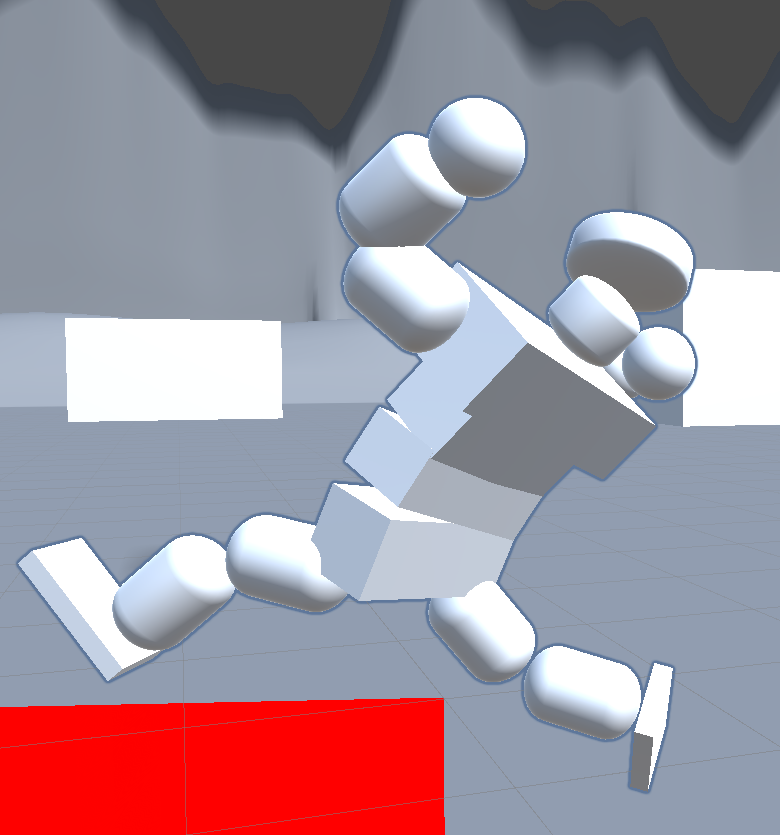
\includegraphics[width=\textwidth]{resources/img/Unity2}
		\caption{Schritt}
		\label{fig:Laufen2}
	\end{subfigure}
	\hfill
	\begin{subfigure}[b]{0.3\textwidth}
		\centering
		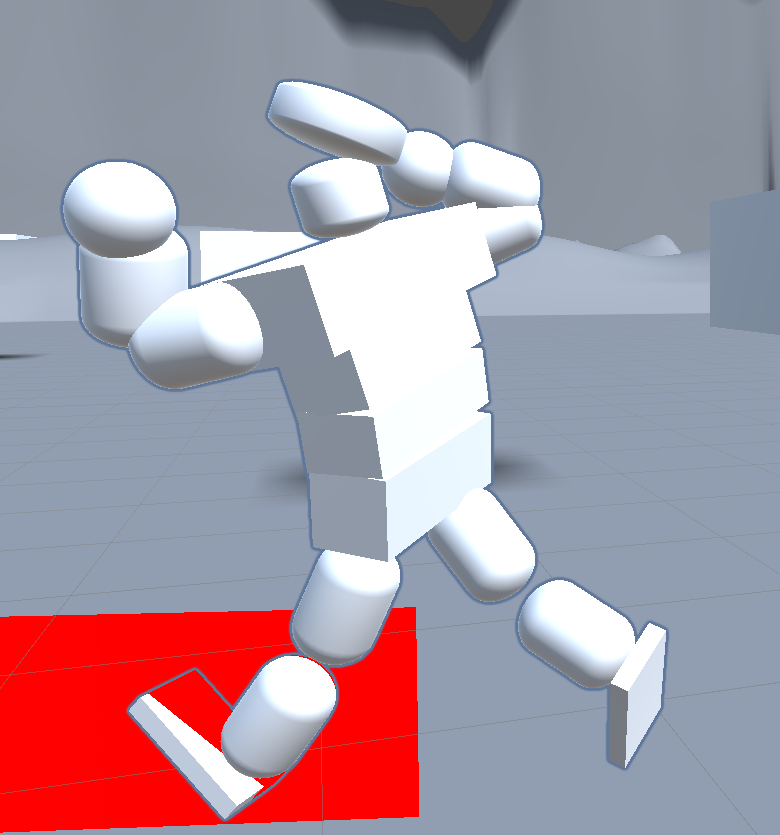
\includegraphics[width=\textwidth]{resources/img/Unity3}
		\caption{Landen}
		\label{fig:Laufen3}
	\end{subfigure}
	\caption{3 Schritte im Laufzyklus eines Zweibeiners.}
	\label{fig:2BLaufen}
\end{figure}

Hier ist zu erkennen, dass es sich nicht um ein Laufen wie bei einem Menschen, welcher ein Fuß auf den Boden stehen hat, den anderen nach vorne zieht und später den zweiten hinter-herzieht, handelt. Sondern es eher einem Rennen gleicht, bei dem beide Beine sich in der Luft befinden. Die Belohnung für das Erreichen der Geschwindigkeit wird hierbei nicht vollständig erreicht und schwankt im Bereich zwischen $0.5$ und $0.6$\footnote{Hier wurden nur die Werte aus dem Log der Belohnungfunktion im Editor abgelesen. Es kann sein, dass die Stichprobe eine Ausnahme abbildet, obwohl diese über mehrere Resets gleich geblieben ist. Eine genauere Untersuchung wäre als Folgearbeit angeraten.}.  Ein weniger trainiert Netzwerk\footnote{Zum Sichttest wurden die Netzwerke \texttt{Generated2B-2000} und \texttt{Generated2B-3000} benutzt. Das erstere ist hierbei das weniger trainierte Netzwerk.} 

Das Laufen ist insbesondere in Kurven instabil. In Abbildung \ref{fig:2bKurve} ist eine Kreatur in einer Kurve abgebildet. Hierbei ist die rote Linie der Pfad bestehend aus Wegpunkten zum Ziel. Der jeweils nächste Punkt ist die Kugel und bildet das Ziel des Agenten ab. Da die Figur mit einer relativ hohen Geschwindigkeit in die Kurve geht und die Stabilität des Laufens dafür nicht ausreicht, springt dieses Ziel häufig in Kurven und trägt so zu der erhöhten Instabilität in Kurven bei.

\begin{figure}
	\centering
	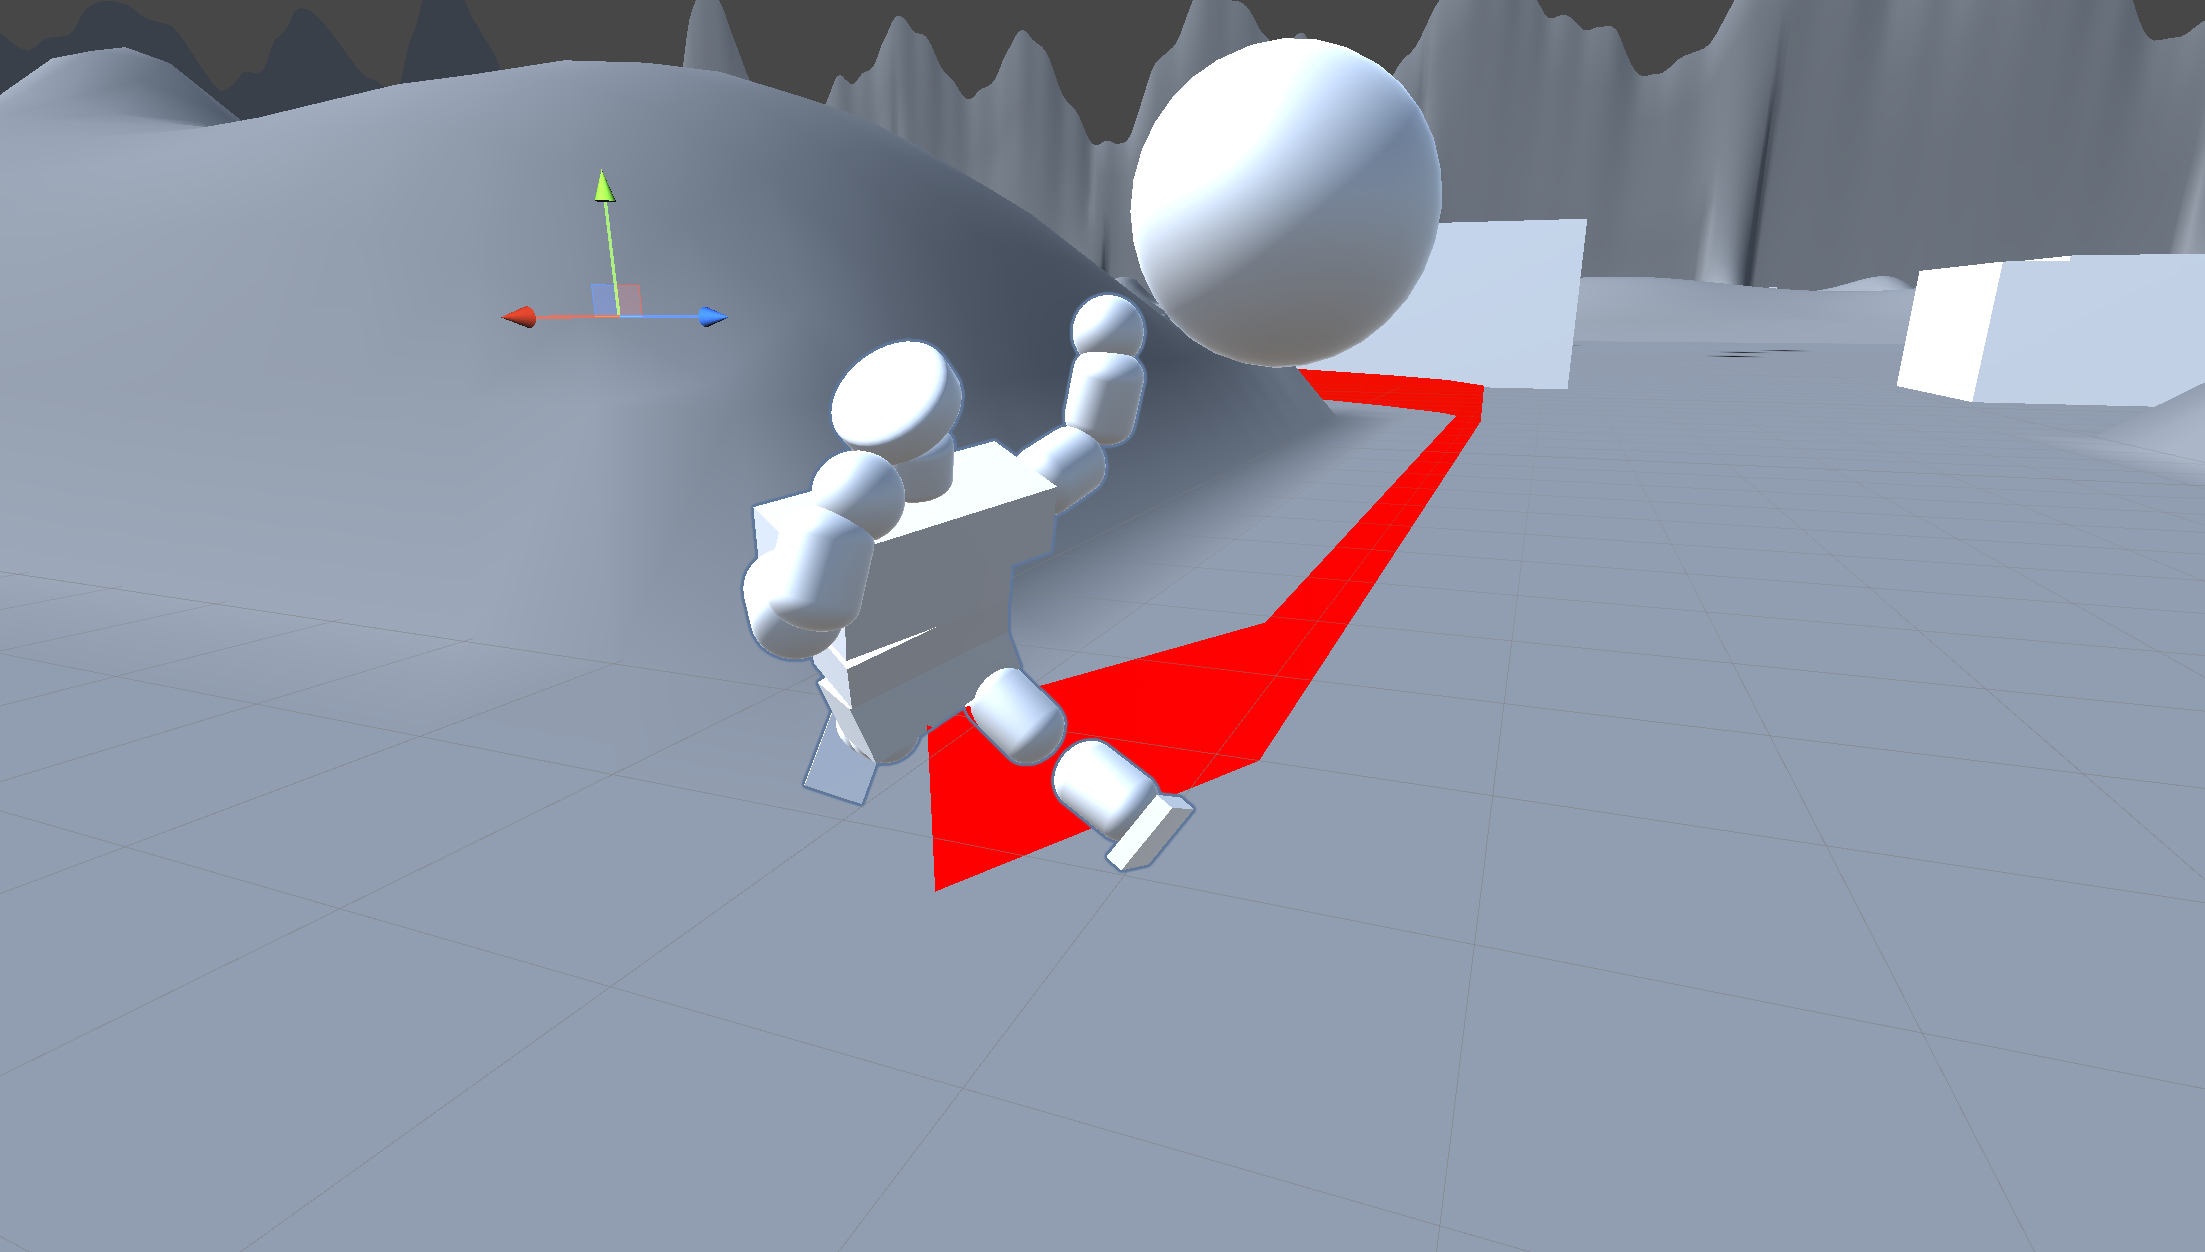
\includegraphics[width=0.7\linewidth]{resources/img/Unity_id9Hnh5u8N}
	\caption[Zweibeiner in einer Kurve]{Die Stabilitätsprobleme eines Zweibeiners in einer Kurve. Hierbei ist die Kugel das aktuell anvisierte Ziel und die rote Linie die Kurve der weiteren Ziele.}
	\label{fig:2bKurve}
\end{figure}

\subsubsection{Aufstehen}

Abbildung \ref{fig:Standup2B_Reward} zeigt die Entwicklung des Rewards während der Updates des Trainingsdurchlaufs. Der Reward steigt in den ersten 1500 bis 2000 Updates kontinuierlich von 0 auf ca. 1200. Danach tritt ein Performance Collapse ein, von dem sich die Policy innerhalb der weiteren berechneten 2000 Updates nur langsam erholt.


\begin{figure}[ht]
    \centering
    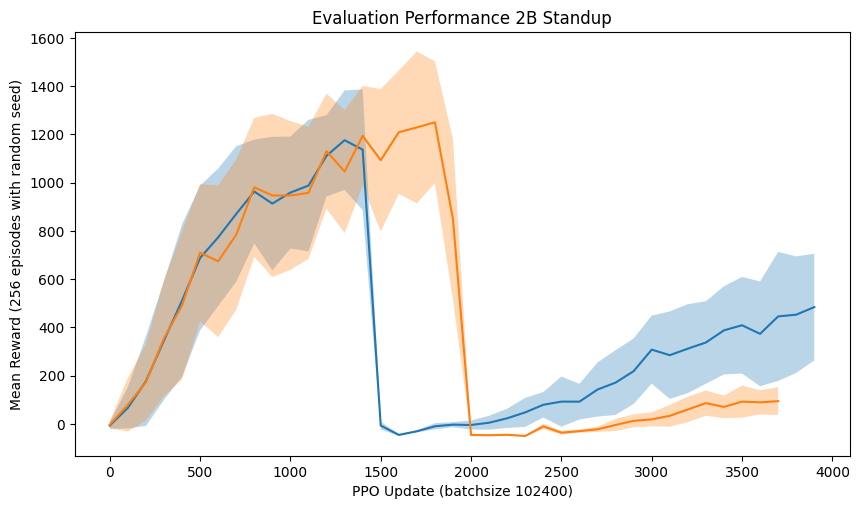
\includegraphics[width=0.5\linewidth]{resources/img/results/Standup2B_Reward.png}
    \caption{Standup 2B Reward}\label{fig:Standup2B_Reward}
\end{figure}

Die Episodenlänge für das Aufstehen der Zweibeiner ist auf 1000 Schritte beschränkt und es gibt keine Bedingung, die den Start einer neuen Episode vor Ablauf der Schritte fordert. Da alle 5 Schritte eine Aktion des Agenten angefordert wird, liegen die in Abbildung \ref{fig:Standup2B_Length} dargestellten Episodenlängen konstant bei 201 Schritten.

\begin{figure}[ht]
    \centering
    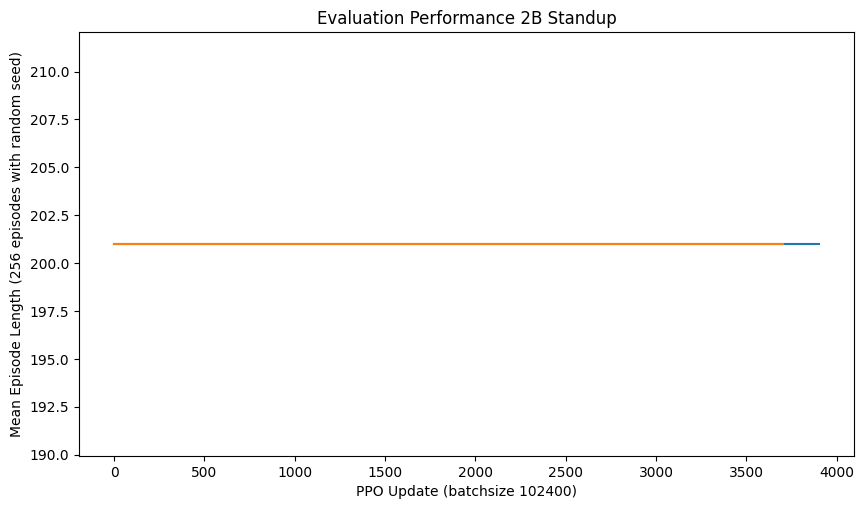
\includegraphics[width=0.5\linewidth]{resources/img/results/Standup2B_Length.png}
    \caption{Standup 2B Length}\label{fig:Standup2B_Length}
\end{figure}

Die Visuelle Evaluation in Unity zeigt, dass selbst die besten Policies (nach 1400 und 1800 Updates) nur in der Lage sind die Kreatur in einer schwungvollen Bewegung aufstehen zu lassen. Die Policies schaffen es allerdings nicht den benötigten Schwung richtig einzuschätzen und daher tritt bei jedem Versuch einer der folgenden Fälle ein.
\begin{itemize}
	\item Sie nimmt zu wenig Schwung und die Kreatur fällt zurück bevor sie aufrecht steht
	\item Sie nimmt zu viel Schwung und schafft es nicht zu stoppen, wodurch die Kreatur wieder umfällt
\end{itemize}
\begin{figure}
	\centering
	\begin{subfigure}[b]{0.2\textwidth}
		\centering
		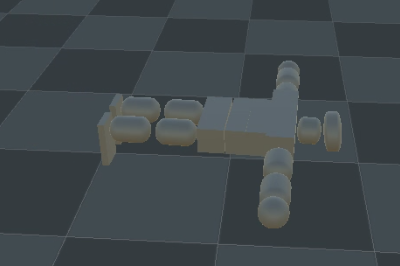
\includegraphics[width=\textwidth]{resources/img/2BAufstehen/Fall1_spawn}
		\caption{Spawn}
	\end{subfigure}
	\hfill
	\begin{subfigure}[b]{0.2\textwidth}
		\centering
		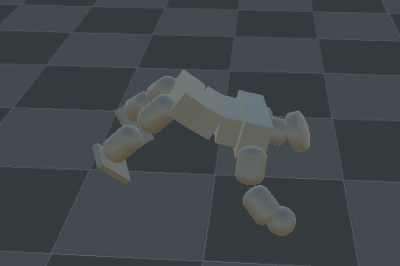
\includegraphics[width=\textwidth]{resources/img/2BAufstehen/Fall1_hoch}
		\caption{Abdrücken}
	\end{subfigure}
	\hfill
	\begin{subfigure}[b]{0.2\textwidth}
		\centering
		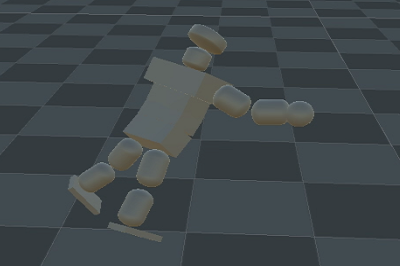
\includegraphics[width=\textwidth]{resources/img/2BAufstehen/Fall1_zenit}
		\caption{Zenit}
	\end{subfigure}
	\hfill
	\begin{subfigure}[b]{0.2\textwidth}
		\centering
		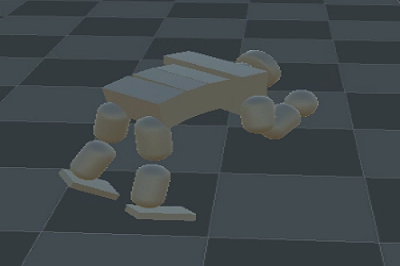
\includegraphics[width=\textwidth]{resources/img/2BAufstehen/Fall1_fallen}
		\caption{Umfallen}
	\end{subfigure}
	\caption{Aufstehen des Zweibeiners: Fall 1}
	\label{fig:2BAufstehen1}
\end{figure}
\begin{figure}
	\centering
	\begin{subfigure}[b]{0.18\textwidth}
		\centering
		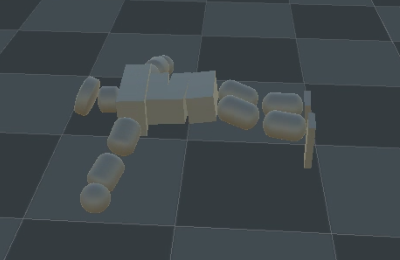
\includegraphics[width=\textwidth]{resources/img/2BAufstehen/Fall2_spawn}
		\caption{Spawn}
	\end{subfigure}
	\hfill
	\begin{subfigure}[b]{0.18\textwidth}
		\centering
		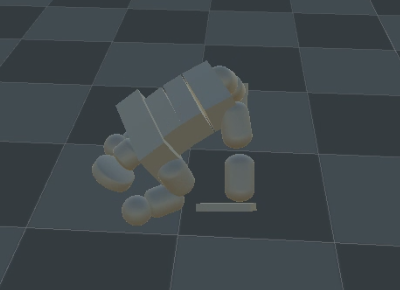
\includegraphics[width=\textwidth]{resources/img/2BAufstehen/Fall2_hoch}
		\caption{Abdrücken}
	\end{subfigure}
	\hfill
	\begin{subfigure}[b]{0.18\textwidth}
		\centering
		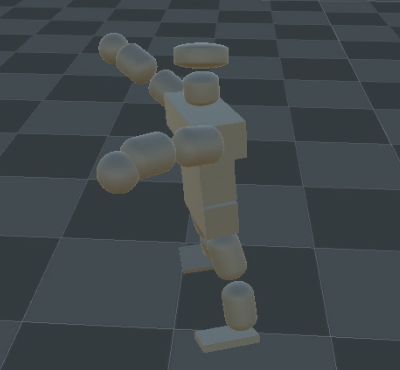
\includegraphics[width=\textwidth]{resources/img/2BAufstehen/Fall2_stehen}
		\caption{Stehen}
	\end{subfigure}
	\hfill
	\begin{subfigure}[b]{0.18\textwidth}
		\centering
		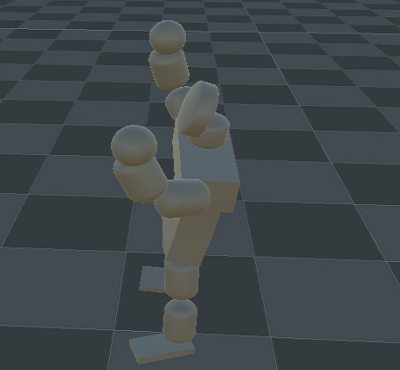
\includegraphics[width=\textwidth]{resources/img/2BAufstehen/Fall2_uber}
		\caption{Umfallen 1}
	\end{subfigure}
	\begin{subfigure}[b]{0.18\textwidth}
	\centering
	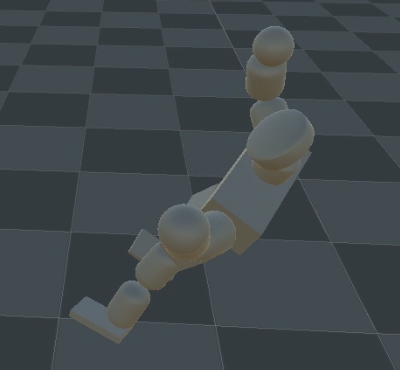
\includegraphics[width=\textwidth]{resources/img/2BAufstehen/Fall2_umfallen}
	\caption{Umfallen 2}
\end{subfigure}
	\caption{Aufstehen des Zweibeiners: Fall 2}
	\label{fig:2BAufstehen2}
\end{figure}
Selbst diese Policies erfüllen also nicht das Ziel eines stabilen Aufstehens der Kreatur.
Die Policies nach dem Performance Collapse führen nur minimal wahrnehmbare Aktionen aus und die Kreatur bleibt unbewegt liegen. 

\section{Probleme}
Bei der Bearbeitung der gegebenen Aufgabenstellung der Projektgruppe haben einige Probleme zu Verzögerungen geführt, welche sich auf die endgültige Funktionalität des Endprodukts ausgewirkt haben.

\subsection{Stabilität des Skeletts}
Das Hauptproblem für die Animatoren-Teilgruppe, welche Hauptsächlich mithilfe von maschinellem Training eine beliebige Kreatur zum laufen bringt, liegt in der Kreaturenstabilität. Zum Anfang der Arbeitsphase wurde die bestehende Walker-Umgebung von Unity analysiert und auf Basis der in dieser Umgebung vorhandenen Kreatur die ersten Tests erstellt. Hierbei konnte verifiziert werden, dass die neu entwickelte Trainingsumgebung funktioniert und die grundlegenden Einstellung zu funktionierenden Ergebnissen führen. Als danach die ersten prozedural generierten Kreaturen eingesetzt wurden, kam es zu einer Vielzahl von Problemen, welche durch andere Defizite in verschiedene Bereichen verstärkt wurden.

\subsubsection{Dokumentation} % Nils
Die meisten Projektgruppenmitglieder hatten vor der PG wenig Erfahrungen mit Unity. Deshalb ist die Dokumentation von Unity eine der wichtigsten Quellen für die Umsetzung der einzelnen Teilprojekte. Die Unity-Dokumentation\footnote{\url{https://docs.unity3d.com/Manual/index.html}} ist Online frei einsehbar für die verschiedenen Versionen der Grafik-Engine. Dabei ist problematisch, dass insbesondere in den Teil zur Physik-Engine oder neueren Pakete ist, welche noch nicht den Vorschau-Status verlassen haben, deutliche Formulierungen fehlen. Ein Beispiel dafür ist die Hilfestellung zur Ragdoll-Stabilität. In einen Nebensatz\footnote{Zu finden auf dieser Unterseite der Dokumentation \url{https://docs.unity3d.com/Manual/RagdollStability.html}} wird erwähnt, dass ein zu großer Massenunterschied zwischen zwei direkt verbundenen Elementen zu unruhigen Ragdolls führen kann. In der Praxis bedeutet dies, dass die generierten Kreaturen bei jegliche Krafteinwirkung explodieren. Eine Fehler-findung und -behebung dieses Problems hat mehrere Wochen gedauert, da die Auswirkungen nur in sehr abgeschwächter Form beschrieben wurden.

Ein weiteres Beispiel ist der \emph{Solver Type}\footnote{Die Komponente der Physikumgebung, welche die Berechnungen für die Kollisionserkennung durchführt.}, welche auf \emph{Projected Gauss Seidel} oder \emph{Temporal Gauss Seidel} gesetzt werden kann. Für das Training wurde in der Anfangsphase versucht jeweils die besten Einstellungen von Unity zu verwenden, was nach Dokumentation die zweitere Option sein sollte. In Gegensatz zu der Dokumentation warnen mehrere Internetquellen\footnote{Siehe beispielsweise das zum PG-Zeitpunkt \href{https://www.youtube.com/watch?v=aZ1zc6zZ61E}{erste Google-Ergebnis}} vor dieser Einstellung. Ein nicht repräsentativer Test hat dies für unsere Kreaturen bestätigt, weshalb im weiteren Verlauf \emph{Projected Gauss Seidel} genutzt wurde. Ein Hinweis, dass \emph{Temporal Gauss Seidel} problematische Ergebnisse produzieren kann, fehlt zum Zeitpunkt des Projetgruppenberichts weiterhin in der Dokumentation.

Insgesamt gab es weitere Beispiele, wie zum Beispiel bei dem \texttt{com.unity.ai.navigation}-Paket \footnote{Eine Dokumentation ist \href{https://docs.unity3d.com/Packages/com.unity.ai.navigation@1.0/manual/NavMeshSurface.html}{hier} zu finden} bei welchem die unterstützten Unity-Versionen unklar ist, welche zusammen zu viel Recherchearbeit geführt haben und deshalb die Bearbeitung der Kernaufgaben verzögert haben.

\subsubsection{Organisatorische Probleme}
Ein weiterer Teilbereich, der zu Verzögerung in den Arbeitsablauf der Animatorenteilgruppe geführt hat, ist organisatorischen Problemen zu zuschrieben. Einige der größten Hindernisse sind die starke Abhängigkeit von den Animatoren und Generatoren, veralte Rechenhardware und fehlender Vorkenntnisse.

Das erste Problem kann wie folgt beschrieben werden. Immer wenn die Änderung an der Kreatur nötig waren, musste das für die Generierung verantwortliche Paket angepasst werden. Inklusive der Kommunikation und der dafür benötigten Arbeitszeit dauerte dies ungefähr eine Woche. In diesen Phasen konnte das Training häufig nicht fortgesetzt werden, da die Kreaturen zu große Fehler hatten. In die andere Richtung konnten die Generatoren nicht weiterarbeiten, da diese auf Feedback von den Trainingsversuchen gewartet haben.

Verstärkt wurde dies durch das zweite Problem. Da LIDO von der ganzen Universität genutzt wird, kann es einige Stunden bis Tage dauern, bis eine Aufgabe abgearbeitet wird. Inklusive der Berechnungszeit des Auftrags konnten so 2 aufeinanderfolgende Experimente gestartet werden je Woche. Da insbesondere in der Mitte der Projektgruppe die Fehler nicht bekannt waren, dauerte das Finden dieser dadurch besonders lange. 
Zusätzlich zu der Wartezeit ist die Rechendauer eines Auftrags auf LIDO für Studenten eingeschränkt. Ein Knoten mit Grafikkarte kann 2 Tage lang reserviert werden. Bei den finalen Training auf einen Knoten des Lehrstuhls stellt sich heraus, dass diese Zeit nicht ausreichend ist, um das (lokale) Maximum der Belohnungsfunktion zu erreichen. Theoretisch wäre ein Fortsetzen der Trainingsaufgabe möglich, führt aber zu eine weiteren Wartezeit auf einen Knoten und Verfälschungen der Trainingsergebnisse durch nicht perfekt zurückgesetzten Parameter des Trainings. 
Des Weiteren stellte sich heraus, dass das Training auf den alten Knoten signifikant länger dauert, als auf den aktuell ausgestatteten Rechenknoten des Lehrstuhls. Ein Trainingsschritt auf den öffentlichen Knoten dauert um die $160 \si{\sec}$  und auf den Lehrstuhlknoten $60 \si{\sec}$. Dies führt zu einer 3-Fachen Wartedauer während der meisten Experimente.

Zuletzt fehlten insbesondere bei dem maschinellen Lernen viele Vorkenntnisse. Das zu Beginn der PG gehaltene Seminar beschäftigte sich mit den eigentlich genutzten Algorithmen, hat aber keine Übersicht über die Forschung im Bereich des physikalischen Laufens gegeben. Hier wurde später \cite{Geijtenbeek2012} genutzt, welches aufgrund des Erscheinungsjahrs kein Überblick für Netzwerkbasierte-Lernmethoden gibt. Eine Einschätzung von weiteren Papieren war dadurch erschwert. Weiterhin beziehen sich viele Arbeiten auf andere Physikumgebgungen, nutzen Imitation zum Lernen oder nutzen explizite Designcharakteristiken der Kreaturen aus\cite{Mourot2022}.

Insgesamt führten die Probleme häufig zu Arbeitsphasen in den die Animatorengruppe oder Generatoren keine neuen Ergebnisse produzieren konnten. In dieser Zeit wurde versucht zukünftige Aufgaben wie beispielsweise eine Generalisierung der Belohnungsfunktionen, eine stärkere anpassbare Trainingsumgebung oder Zusatzfunktionen wie ein unebener Boden. Durch die grundlegenden Probleme bei der Stabilität konnte am Ende keine dieser Erweiterungen fertiggestellt werden.

\section{Diskussion}
\label{Diskussion}

Dieser Abschnitt diskutiert die zuvor beschriebenen Ergebnisse der Projektgruppe im Bezug zur initialen Zielsetzung \ref{Zielsetzung_und_Vorgehensweise}.

\paragraph{Die Generierung von Spielleveln}

\paragraph{Generierung der Monster}

\paragraph{Fortbewegung der Monster}

